% Created by tikzDevice version 0.12.3.1 on 2021-12-03 16:19:11
% !TEX encoding = UTF-8 Unicode
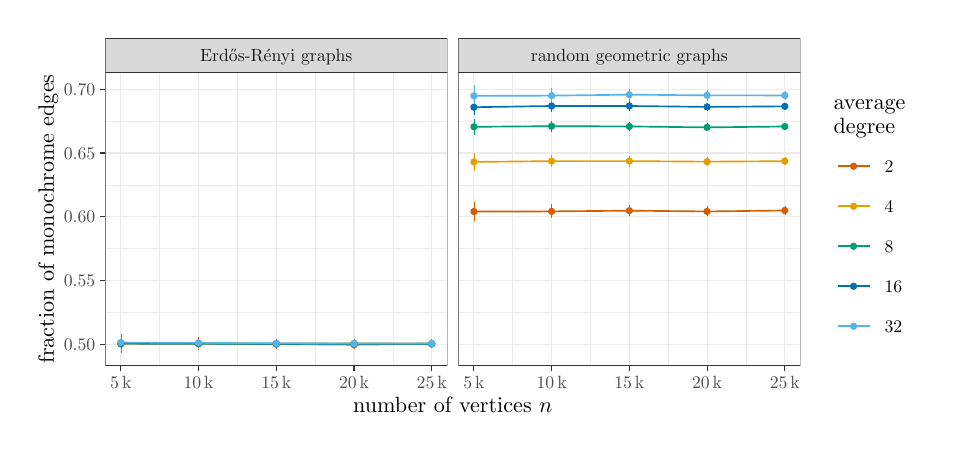
\begin{tikzpicture}[x=1pt,y=1pt]
\definecolor{fillColor}{RGB}{255,255,255}
\path[use as bounding box,fill=fillColor,fill opacity=0.00] (0,0) rectangle (325.21,144.54);
\begin{scope}
\path[clip] (  0.00,  0.00) rectangle (325.21,144.54);
\definecolor{drawColor}{RGB}{255,255,255}
\definecolor{fillColor}{RGB}{255,255,255}

\path[draw=drawColor,line width= 0.4pt,line join=round,line cap=round,fill=fillColor] (  0.00,  0.00) rectangle (325.21,144.54);
\end{scope}
\begin{scope}
\path[clip] ( 28.04, 22.32) rectangle (151.62,128.49);
\definecolor{fillColor}{RGB}{255,255,255}

\path[fill=fillColor] ( 28.04, 22.32) rectangle (151.62,128.49);
\definecolor{drawColor}{gray}{0.92}

\path[draw=drawColor,line width= 0.2pt,line join=round] ( 28.04, 41.72) --
	(151.62, 41.72);

\path[draw=drawColor,line width= 0.2pt,line join=round] ( 28.04, 64.73) --
	(151.62, 64.73);

\path[draw=drawColor,line width= 0.2pt,line join=round] ( 28.04, 87.74) --
	(151.62, 87.74);

\path[draw=drawColor,line width= 0.2pt,line join=round] ( 28.04,110.75) --
	(151.62,110.75);

\path[draw=drawColor,line width= 0.2pt,line join=round] ( 47.70, 22.32) --
	( 47.70,128.49);

\path[draw=drawColor,line width= 0.2pt,line join=round] ( 75.79, 22.32) --
	( 75.79,128.49);

\path[draw=drawColor,line width= 0.2pt,line join=round] (103.87, 22.32) --
	(103.87,128.49);

\path[draw=drawColor,line width= 0.2pt,line join=round] (131.96, 22.32) --
	(131.96,128.49);

\path[draw=drawColor,line width= 0.4pt,line join=round] ( 28.04, 30.21) --
	(151.62, 30.21);

\path[draw=drawColor,line width= 0.4pt,line join=round] ( 28.04, 53.22) --
	(151.62, 53.22);

\path[draw=drawColor,line width= 0.4pt,line join=round] ( 28.04, 76.24) --
	(151.62, 76.24);

\path[draw=drawColor,line width= 0.4pt,line join=round] ( 28.04, 99.25) --
	(151.62, 99.25);

\path[draw=drawColor,line width= 0.4pt,line join=round] ( 28.04,122.26) --
	(151.62,122.26);

\path[draw=drawColor,line width= 0.4pt,line join=round] ( 33.66, 22.32) --
	( 33.66,128.49);

\path[draw=drawColor,line width= 0.4pt,line join=round] ( 61.74, 22.32) --
	( 61.74,128.49);

\path[draw=drawColor,line width= 0.4pt,line join=round] ( 89.83, 22.32) --
	( 89.83,128.49);

\path[draw=drawColor,line width= 0.4pt,line join=round] (117.92, 22.32) --
	(117.92,128.49);

\path[draw=drawColor,line width= 0.4pt,line join=round] (146.00, 22.32) --
	(146.00,128.49);
\definecolor{drawColor}{RGB}{213,94,0}

\path[draw=drawColor,line width= 0.2pt,line join=round] ( 33.66, 33.88) --
	( 33.66, 33.88);

\path[draw=drawColor,line width= 0.2pt,line join=round] ( 33.66, 33.88) --
	( 33.66, 27.14);

\path[draw=drawColor,line width= 0.2pt,line join=round] ( 33.66, 27.14) --
	( 33.66, 27.14);

\path[draw=drawColor,line width= 0.2pt,line join=round] ( 61.74, 32.90) --
	( 61.74, 32.90);

\path[draw=drawColor,line width= 0.2pt,line join=round] ( 61.74, 32.90) --
	( 61.74, 27.95);

\path[draw=drawColor,line width= 0.2pt,line join=round] ( 61.74, 27.95) --
	( 61.74, 27.95);

\path[draw=drawColor,line width= 0.2pt,line join=round] ( 89.83, 32.15) --
	( 89.83, 32.15);

\path[draw=drawColor,line width= 0.2pt,line join=round] ( 89.83, 32.15) --
	( 89.83, 28.46);

\path[draw=drawColor,line width= 0.2pt,line join=round] ( 89.83, 28.46) --
	( 89.83, 28.46);

\path[draw=drawColor,line width= 0.2pt,line join=round] (117.92, 31.91) --
	(117.92, 31.91);

\path[draw=drawColor,line width= 0.2pt,line join=round] (117.92, 31.91) --
	(117.92, 28.37);

\path[draw=drawColor,line width= 0.2pt,line join=round] (117.92, 28.37) --
	(117.92, 28.37);

\path[draw=drawColor,line width= 0.2pt,line join=round] (146.00, 31.90) --
	(146.00, 31.90);

\path[draw=drawColor,line width= 0.2pt,line join=round] (146.00, 31.90) --
	(146.00, 28.66);

\path[draw=drawColor,line width= 0.2pt,line join=round] (146.00, 28.66) --
	(146.00, 28.66);
\definecolor{drawColor}{RGB}{230,159,0}

\path[draw=drawColor,line width= 0.2pt,line join=round] ( 33.66, 32.94) --
	( 33.66, 32.94);

\path[draw=drawColor,line width= 0.2pt,line join=round] ( 33.66, 32.94) --
	( 33.66, 28.18);

\path[draw=drawColor,line width= 0.2pt,line join=round] ( 33.66, 28.18) --
	( 33.66, 28.18);

\path[draw=drawColor,line width= 0.2pt,line join=round] ( 61.74, 32.04) --
	( 61.74, 32.04);

\path[draw=drawColor,line width= 0.2pt,line join=round] ( 61.74, 32.04) --
	( 61.74, 28.44);

\path[draw=drawColor,line width= 0.2pt,line join=round] ( 61.74, 28.44) --
	( 61.74, 28.44);

\path[draw=drawColor,line width= 0.2pt,line join=round] ( 89.83, 31.68) --
	( 89.83, 31.68);

\path[draw=drawColor,line width= 0.2pt,line join=round] ( 89.83, 31.68) --
	( 89.83, 28.78);

\path[draw=drawColor,line width= 0.2pt,line join=round] ( 89.83, 28.78) --
	( 89.83, 28.78);

\path[draw=drawColor,line width= 0.2pt,line join=round] (117.92, 31.68) --
	(117.92, 31.68);

\path[draw=drawColor,line width= 0.2pt,line join=round] (117.92, 31.68) --
	(117.92, 28.96);

\path[draw=drawColor,line width= 0.2pt,line join=round] (117.92, 28.96) --
	(117.92, 28.96);

\path[draw=drawColor,line width= 0.2pt,line join=round] (146.00, 31.45) --
	(146.00, 31.45);

\path[draw=drawColor,line width= 0.2pt,line join=round] (146.00, 31.45) --
	(146.00, 29.22);

\path[draw=drawColor,line width= 0.2pt,line join=round] (146.00, 29.22) --
	(146.00, 29.22);
\definecolor{drawColor}{RGB}{0,158,115}

\path[draw=drawColor,line width= 0.2pt,line join=round] ( 33.66, 32.28) --
	( 33.66, 32.28);

\path[draw=drawColor,line width= 0.2pt,line join=round] ( 33.66, 32.28) --
	( 33.66, 28.33);

\path[draw=drawColor,line width= 0.2pt,line join=round] ( 33.66, 28.33) --
	( 33.66, 28.33);

\path[draw=drawColor,line width= 0.2pt,line join=round] ( 61.74, 31.73) --
	( 61.74, 31.73);

\path[draw=drawColor,line width= 0.2pt,line join=round] ( 61.74, 31.73) --
	( 61.74, 28.94);

\path[draw=drawColor,line width= 0.2pt,line join=round] ( 61.74, 28.94) --
	( 61.74, 28.94);

\path[draw=drawColor,line width= 0.2pt,line join=round] ( 89.83, 31.29) --
	( 89.83, 31.29);

\path[draw=drawColor,line width= 0.2pt,line join=round] ( 89.83, 31.29) --
	( 89.83, 29.24);

\path[draw=drawColor,line width= 0.2pt,line join=round] ( 89.83, 29.24) --
	( 89.83, 29.24);

\path[draw=drawColor,line width= 0.2pt,line join=round] (117.92, 31.21) --
	(117.92, 31.21);

\path[draw=drawColor,line width= 0.2pt,line join=round] (117.92, 31.21) --
	(117.92, 29.44);

\path[draw=drawColor,line width= 0.2pt,line join=round] (117.92, 29.44) --
	(117.92, 29.44);

\path[draw=drawColor,line width= 0.2pt,line join=round] (146.00, 31.06) --
	(146.00, 31.06);

\path[draw=drawColor,line width= 0.2pt,line join=round] (146.00, 31.06) --
	(146.00, 29.44);

\path[draw=drawColor,line width= 0.2pt,line join=round] (146.00, 29.44) --
	(146.00, 29.44);
\definecolor{drawColor}{RGB}{0,114,178}

\path[draw=drawColor,line width= 0.2pt,line join=round] ( 33.66, 31.94) --
	( 33.66, 31.94);

\path[draw=drawColor,line width= 0.2pt,line join=round] ( 33.66, 31.94) --
	( 33.66, 29.05);

\path[draw=drawColor,line width= 0.2pt,line join=round] ( 33.66, 29.05) --
	( 33.66, 29.05);

\path[draw=drawColor,line width= 0.2pt,line join=round] ( 61.74, 31.41) --
	( 61.74, 31.41);

\path[draw=drawColor,line width= 0.2pt,line join=round] ( 61.74, 31.41) --
	( 61.74, 29.35);

\path[draw=drawColor,line width= 0.2pt,line join=round] ( 61.74, 29.35) --
	( 61.74, 29.35);

\path[draw=drawColor,line width= 0.2pt,line join=round] ( 89.83, 31.09) --
	( 89.83, 31.09);

\path[draw=drawColor,line width= 0.2pt,line join=round] ( 89.83, 31.09) --
	( 89.83, 29.55);

\path[draw=drawColor,line width= 0.2pt,line join=round] ( 89.83, 29.55) --
	( 89.83, 29.55);

\path[draw=drawColor,line width= 0.2pt,line join=round] (117.92, 30.86) --
	(117.92, 30.86);

\path[draw=drawColor,line width= 0.2pt,line join=round] (117.92, 30.86) --
	(117.92, 29.60);

\path[draw=drawColor,line width= 0.2pt,line join=round] (117.92, 29.60) --
	(117.92, 29.60);

\path[draw=drawColor,line width= 0.2pt,line join=round] (146.00, 30.90) --
	(146.00, 30.90);

\path[draw=drawColor,line width= 0.2pt,line join=round] (146.00, 30.90) --
	(146.00, 29.71);

\path[draw=drawColor,line width= 0.2pt,line join=round] (146.00, 29.71) --
	(146.00, 29.71);
\definecolor{drawColor}{RGB}{86,180,233}

\path[draw=drawColor,line width= 0.2pt,line join=round] ( 33.66, 32.01) --
	( 33.66, 32.01);

\path[draw=drawColor,line width= 0.2pt,line join=round] ( 33.66, 32.01) --
	( 33.66, 29.70);

\path[draw=drawColor,line width= 0.2pt,line join=round] ( 33.66, 29.70) --
	( 33.66, 29.70);

\path[draw=drawColor,line width= 0.2pt,line join=round] ( 61.74, 31.42) --
	( 61.74, 31.42);

\path[draw=drawColor,line width= 0.2pt,line join=round] ( 61.74, 31.42) --
	( 61.74, 29.85);

\path[draw=drawColor,line width= 0.2pt,line join=round] ( 61.74, 29.85) --
	( 61.74, 29.85);

\path[draw=drawColor,line width= 0.2pt,line join=round] ( 89.83, 31.08) --
	( 89.83, 31.08);

\path[draw=drawColor,line width= 0.2pt,line join=round] ( 89.83, 31.08) --
	( 89.83, 29.86);

\path[draw=drawColor,line width= 0.2pt,line join=round] ( 89.83, 29.86) --
	( 89.83, 29.86);

\path[draw=drawColor,line width= 0.2pt,line join=round] (117.92, 30.91) --
	(117.92, 30.91);

\path[draw=drawColor,line width= 0.2pt,line join=round] (117.92, 30.91) --
	(117.92, 29.88);

\path[draw=drawColor,line width= 0.2pt,line join=round] (117.92, 29.88) --
	(117.92, 29.88);

\path[draw=drawColor,line width= 0.2pt,line join=round] (146.00, 30.88) --
	(146.00, 30.88);

\path[draw=drawColor,line width= 0.2pt,line join=round] (146.00, 30.88) --
	(146.00, 29.92);

\path[draw=drawColor,line width= 0.2pt,line join=round] (146.00, 29.92) --
	(146.00, 29.92);
\definecolor{drawColor}{RGB}{213,94,0}

\path[draw=drawColor,line width= 0.6pt,line join=round] ( 33.66, 30.44) --
	( 61.74, 30.47) --
	( 89.83, 30.21) --
	(117.92, 29.97) --
	(146.00, 30.32);
\definecolor{drawColor}{RGB}{230,159,0}

\path[draw=drawColor,line width= 0.6pt,line join=round] ( 33.66, 30.36) --
	( 61.74, 30.33) --
	( 89.83, 30.29) --
	(117.92, 30.41) --
	(146.00, 30.41);
\definecolor{drawColor}{RGB}{0,158,115}

\path[draw=drawColor,line width= 0.6pt,line join=round] ( 33.66, 30.36) --
	( 61.74, 30.37) --
	( 89.83, 30.30) --
	(117.92, 30.34) --
	(146.00, 30.25);
\definecolor{drawColor}{RGB}{0,114,178}

\path[draw=drawColor,line width= 0.6pt,line join=round] ( 33.66, 30.46) --
	( 61.74, 30.39) --
	( 89.83, 30.33) --
	(117.92, 30.28) --
	(146.00, 30.30);
\definecolor{drawColor}{RGB}{86,180,233}

\path[draw=drawColor,line width= 0.6pt,line join=round] ( 33.66, 30.76) --
	( 61.74, 30.64) --
	( 89.83, 30.47) --
	(117.92, 30.39) --
	(146.00, 30.39);
\definecolor{drawColor}{RGB}{213,94,0}
\definecolor{fillColor}{RGB}{213,94,0}

\path[draw=drawColor,line width= 0.4pt,line join=round,line cap=round,fill=fillColor] ( 33.66, 30.44) circle (  1.11);

\path[draw=drawColor,line width= 0.4pt,line join=round,line cap=round,fill=fillColor] ( 61.74, 30.47) circle (  1.11);

\path[draw=drawColor,line width= 0.4pt,line join=round,line cap=round,fill=fillColor] ( 89.83, 30.21) circle (  1.11);

\path[draw=drawColor,line width= 0.4pt,line join=round,line cap=round,fill=fillColor] (117.92, 29.97) circle (  1.11);

\path[draw=drawColor,line width= 0.4pt,line join=round,line cap=round,fill=fillColor] (146.00, 30.32) circle (  1.11);
\definecolor{drawColor}{RGB}{230,159,0}
\definecolor{fillColor}{RGB}{230,159,0}

\path[draw=drawColor,line width= 0.4pt,line join=round,line cap=round,fill=fillColor] ( 33.66, 30.36) circle (  1.11);

\path[draw=drawColor,line width= 0.4pt,line join=round,line cap=round,fill=fillColor] ( 61.74, 30.33) circle (  1.11);

\path[draw=drawColor,line width= 0.4pt,line join=round,line cap=round,fill=fillColor] ( 89.83, 30.29) circle (  1.11);

\path[draw=drawColor,line width= 0.4pt,line join=round,line cap=round,fill=fillColor] (117.92, 30.41) circle (  1.11);

\path[draw=drawColor,line width= 0.4pt,line join=round,line cap=round,fill=fillColor] (146.00, 30.41) circle (  1.11);
\definecolor{drawColor}{RGB}{0,158,115}
\definecolor{fillColor}{RGB}{0,158,115}

\path[draw=drawColor,line width= 0.4pt,line join=round,line cap=round,fill=fillColor] ( 33.66, 30.36) circle (  1.11);

\path[draw=drawColor,line width= 0.4pt,line join=round,line cap=round,fill=fillColor] ( 61.74, 30.37) circle (  1.11);

\path[draw=drawColor,line width= 0.4pt,line join=round,line cap=round,fill=fillColor] ( 89.83, 30.30) circle (  1.11);

\path[draw=drawColor,line width= 0.4pt,line join=round,line cap=round,fill=fillColor] (117.92, 30.34) circle (  1.11);

\path[draw=drawColor,line width= 0.4pt,line join=round,line cap=round,fill=fillColor] (146.00, 30.25) circle (  1.11);
\definecolor{drawColor}{RGB}{0,114,178}
\definecolor{fillColor}{RGB}{0,114,178}

\path[draw=drawColor,line width= 0.4pt,line join=round,line cap=round,fill=fillColor] ( 33.66, 30.46) circle (  1.11);

\path[draw=drawColor,line width= 0.4pt,line join=round,line cap=round,fill=fillColor] ( 61.74, 30.39) circle (  1.11);

\path[draw=drawColor,line width= 0.4pt,line join=round,line cap=round,fill=fillColor] ( 89.83, 30.33) circle (  1.11);

\path[draw=drawColor,line width= 0.4pt,line join=round,line cap=round,fill=fillColor] (117.92, 30.28) circle (  1.11);

\path[draw=drawColor,line width= 0.4pt,line join=round,line cap=round,fill=fillColor] (146.00, 30.30) circle (  1.11);
\definecolor{drawColor}{RGB}{86,180,233}
\definecolor{fillColor}{RGB}{86,180,233}

\path[draw=drawColor,line width= 0.4pt,line join=round,line cap=round,fill=fillColor] ( 33.66, 30.76) circle (  1.11);

\path[draw=drawColor,line width= 0.4pt,line join=round,line cap=round,fill=fillColor] ( 61.74, 30.64) circle (  1.11);

\path[draw=drawColor,line width= 0.4pt,line join=round,line cap=round,fill=fillColor] ( 89.83, 30.47) circle (  1.11);

\path[draw=drawColor,line width= 0.4pt,line join=round,line cap=round,fill=fillColor] (117.92, 30.39) circle (  1.11);

\path[draw=drawColor,line width= 0.4pt,line join=round,line cap=round,fill=fillColor] (146.00, 30.39) circle (  1.11);
\definecolor{drawColor}{gray}{0.20}

\path[draw=drawColor,line width= 0.4pt,line join=round,line cap=round] ( 28.04, 22.32) rectangle (151.62,128.49);
\end{scope}
\begin{scope}
\path[clip] (155.62, 22.32) rectangle (279.20,128.49);
\definecolor{fillColor}{RGB}{255,255,255}

\path[fill=fillColor] (155.62, 22.32) rectangle (279.20,128.49);
\definecolor{drawColor}{gray}{0.92}

\path[draw=drawColor,line width= 0.2pt,line join=round] (155.62, 41.72) --
	(279.20, 41.72);

\path[draw=drawColor,line width= 0.2pt,line join=round] (155.62, 64.73) --
	(279.20, 64.73);

\path[draw=drawColor,line width= 0.2pt,line join=round] (155.62, 87.74) --
	(279.20, 87.74);

\path[draw=drawColor,line width= 0.2pt,line join=round] (155.62,110.75) --
	(279.20,110.75);

\path[draw=drawColor,line width= 0.2pt,line join=round] (175.28, 22.32) --
	(175.28,128.49);

\path[draw=drawColor,line width= 0.2pt,line join=round] (203.37, 22.32) --
	(203.37,128.49);

\path[draw=drawColor,line width= 0.2pt,line join=round] (231.45, 22.32) --
	(231.45,128.49);

\path[draw=drawColor,line width= 0.2pt,line join=round] (259.54, 22.32) --
	(259.54,128.49);

\path[draw=drawColor,line width= 0.4pt,line join=round] (155.62, 30.21) --
	(279.20, 30.21);

\path[draw=drawColor,line width= 0.4pt,line join=round] (155.62, 53.22) --
	(279.20, 53.22);

\path[draw=drawColor,line width= 0.4pt,line join=round] (155.62, 76.24) --
	(279.20, 76.24);

\path[draw=drawColor,line width= 0.4pt,line join=round] (155.62, 99.25) --
	(279.20, 99.25);

\path[draw=drawColor,line width= 0.4pt,line join=round] (155.62,122.26) --
	(279.20,122.26);

\path[draw=drawColor,line width= 0.4pt,line join=round] (161.24, 22.32) --
	(161.24,128.49);

\path[draw=drawColor,line width= 0.4pt,line join=round] (189.32, 22.32) --
	(189.32,128.49);

\path[draw=drawColor,line width= 0.4pt,line join=round] (217.41, 22.32) --
	(217.41,128.49);

\path[draw=drawColor,line width= 0.4pt,line join=round] (245.50, 22.32) --
	(245.50,128.49);

\path[draw=drawColor,line width= 0.4pt,line join=round] (273.58, 22.32) --
	(273.58,128.49);
\definecolor{drawColor}{RGB}{213,94,0}

\path[draw=drawColor,line width= 0.2pt,line join=round] (161.24, 81.72) --
	(161.24, 81.72);

\path[draw=drawColor,line width= 0.2pt,line join=round] (161.24, 81.72) --
	(161.24, 74.65);

\path[draw=drawColor,line width= 0.2pt,line join=round] (161.24, 74.65) --
	(161.24, 74.65);

\path[draw=drawColor,line width= 0.2pt,line join=round] (189.32, 80.87) --
	(189.32, 80.87);

\path[draw=drawColor,line width= 0.2pt,line join=round] (189.32, 80.87) --
	(189.32, 75.64);

\path[draw=drawColor,line width= 0.2pt,line join=round] (189.32, 75.64) --
	(189.32, 75.64);

\path[draw=drawColor,line width= 0.2pt,line join=round] (217.41, 80.63) --
	(217.41, 80.63);

\path[draw=drawColor,line width= 0.2pt,line join=round] (217.41, 80.63) --
	(217.41, 76.34);

\path[draw=drawColor,line width= 0.2pt,line join=round] (217.41, 76.34) --
	(217.41, 76.34);

\path[draw=drawColor,line width= 0.2pt,line join=round] (245.50, 80.06) --
	(245.50, 80.06);

\path[draw=drawColor,line width= 0.2pt,line join=round] (245.50, 80.06) --
	(245.50, 76.51);

\path[draw=drawColor,line width= 0.2pt,line join=round] (245.50, 76.51) --
	(245.50, 76.51);

\path[draw=drawColor,line width= 0.2pt,line join=round] (273.58, 79.98) --
	(273.58, 79.98);

\path[draw=drawColor,line width= 0.2pt,line join=round] (273.58, 79.98) --
	(273.58, 76.91);

\path[draw=drawColor,line width= 0.2pt,line join=round] (273.58, 76.91) --
	(273.58, 76.91);
\definecolor{drawColor}{RGB}{230,159,0}

\path[draw=drawColor,line width= 0.2pt,line join=round] (161.24, 99.28) --
	(161.24, 99.28);

\path[draw=drawColor,line width= 0.2pt,line join=round] (161.24, 99.28) --
	(161.24, 92.87);

\path[draw=drawColor,line width= 0.2pt,line join=round] (161.24, 92.87) --
	(161.24, 92.87);

\path[draw=drawColor,line width= 0.2pt,line join=round] (189.32, 98.49) --
	(189.32, 98.49);

\path[draw=drawColor,line width= 0.2pt,line join=round] (189.32, 98.49) --
	(189.32, 94.02);

\path[draw=drawColor,line width= 0.2pt,line join=round] (189.32, 94.02) --
	(189.32, 94.02);

\path[draw=drawColor,line width= 0.2pt,line join=round] (217.41, 97.99) --
	(217.41, 97.99);

\path[draw=drawColor,line width= 0.2pt,line join=round] (217.41, 97.99) --
	(217.41, 94.35);

\path[draw=drawColor,line width= 0.2pt,line join=round] (217.41, 94.35) --
	(217.41, 94.35);

\path[draw=drawColor,line width= 0.2pt,line join=round] (245.50, 97.64) --
	(245.50, 97.64);

\path[draw=drawColor,line width= 0.2pt,line join=round] (245.50, 97.64) --
	(245.50, 94.60);

\path[draw=drawColor,line width= 0.2pt,line join=round] (245.50, 94.60) --
	(245.50, 94.60);

\path[draw=drawColor,line width= 0.2pt,line join=round] (273.58, 97.79) --
	(273.58, 97.79);

\path[draw=drawColor,line width= 0.2pt,line join=round] (273.58, 97.79) --
	(273.58, 94.94);

\path[draw=drawColor,line width= 0.2pt,line join=round] (273.58, 94.94) --
	(273.58, 94.94);
\definecolor{drawColor}{RGB}{0,158,115}

\path[draw=drawColor,line width= 0.2pt,line join=round] (161.24,111.65) --
	(161.24,111.65);

\path[draw=drawColor,line width= 0.2pt,line join=round] (161.24,111.65) --
	(161.24,105.83);

\path[draw=drawColor,line width= 0.2pt,line join=round] (161.24,105.83) --
	(161.24,105.83);

\path[draw=drawColor,line width= 0.2pt,line join=round] (189.32,110.93) --
	(189.32,110.93);

\path[draw=drawColor,line width= 0.2pt,line join=round] (189.32,110.93) --
	(189.32,106.76);

\path[draw=drawColor,line width= 0.2pt,line join=round] (189.32,106.76) --
	(189.32,106.76);

\path[draw=drawColor,line width= 0.2pt,line join=round] (217.41,110.63) --
	(217.41,110.63);

\path[draw=drawColor,line width= 0.2pt,line join=round] (217.41,110.63) --
	(217.41,107.16);

\path[draw=drawColor,line width= 0.2pt,line join=round] (217.41,107.16) --
	(217.41,107.16);

\path[draw=drawColor,line width= 0.2pt,line join=round] (245.50,110.04) --
	(245.50,110.04);

\path[draw=drawColor,line width= 0.2pt,line join=round] (245.50,110.04) --
	(245.50,107.09);

\path[draw=drawColor,line width= 0.2pt,line join=round] (245.50,107.09) --
	(245.50,107.09);

\path[draw=drawColor,line width= 0.2pt,line join=round] (273.58,110.05) --
	(273.58,110.05);

\path[draw=drawColor,line width= 0.2pt,line join=round] (273.58,110.05) --
	(273.58,107.44);

\path[draw=drawColor,line width= 0.2pt,line join=round] (273.58,107.44) --
	(273.58,107.44);
\definecolor{drawColor}{RGB}{0,114,178}

\path[draw=drawColor,line width= 0.2pt,line join=round] (161.24,119.01) --
	(161.24,119.01);

\path[draw=drawColor,line width= 0.2pt,line join=round] (161.24,119.01) --
	(161.24,112.85);

\path[draw=drawColor,line width= 0.2pt,line join=round] (161.24,112.85) --
	(161.24,112.85);

\path[draw=drawColor,line width= 0.2pt,line join=round] (189.32,118.44) --
	(189.32,118.44);

\path[draw=drawColor,line width= 0.2pt,line join=round] (189.32,118.44) --
	(189.32,114.03);

\path[draw=drawColor,line width= 0.2pt,line join=round] (189.32,114.03) --
	(189.32,114.03);

\path[draw=drawColor,line width= 0.2pt,line join=round] (217.41,118.24) --
	(217.41,118.24);

\path[draw=drawColor,line width= 0.2pt,line join=round] (217.41,118.24) --
	(217.41,114.52);

\path[draw=drawColor,line width= 0.2pt,line join=round] (217.41,114.52) --
	(217.41,114.52);

\path[draw=drawColor,line width= 0.2pt,line join=round] (245.50,117.41) --
	(245.50,117.41);

\path[draw=drawColor,line width= 0.2pt,line join=round] (245.50,117.41) --
	(245.50,114.57);

\path[draw=drawColor,line width= 0.2pt,line join=round] (245.50,114.57) --
	(245.50,114.57);

\path[draw=drawColor,line width= 0.2pt,line join=round] (273.58,117.44) --
	(273.58,117.44);

\path[draw=drawColor,line width= 0.2pt,line join=round] (273.58,117.44) --
	(273.58,114.71);

\path[draw=drawColor,line width= 0.2pt,line join=round] (273.58,114.71) --
	(273.58,114.71);
\definecolor{drawColor}{RGB}{86,180,233}

\path[draw=drawColor,line width= 0.2pt,line join=round] (161.24,123.66) --
	(161.24,123.66);

\path[draw=drawColor,line width= 0.2pt,line join=round] (161.24,123.66) --
	(161.24,116.31);

\path[draw=drawColor,line width= 0.2pt,line join=round] (161.24,116.31) --
	(161.24,116.31);

\path[draw=drawColor,line width= 0.2pt,line join=round] (189.32,122.69) --
	(189.32,122.69);

\path[draw=drawColor,line width= 0.2pt,line join=round] (189.32,122.69) --
	(189.32,117.31);

\path[draw=drawColor,line width= 0.2pt,line join=round] (189.32,117.31) --
	(189.32,117.31);

\path[draw=drawColor,line width= 0.2pt,line join=round] (217.41,122.42) --
	(217.41,122.42);

\path[draw=drawColor,line width= 0.2pt,line join=round] (217.41,122.42) --
	(217.41,118.10);

\path[draw=drawColor,line width= 0.2pt,line join=round] (217.41,118.10) --
	(217.41,118.10);

\path[draw=drawColor,line width= 0.2pt,line join=round] (245.50,121.89) --
	(245.50,121.89);

\path[draw=drawColor,line width= 0.2pt,line join=round] (245.50,121.89) --
	(245.50,118.22);

\path[draw=drawColor,line width= 0.2pt,line join=round] (245.50,118.22) --
	(245.50,118.22);

\path[draw=drawColor,line width= 0.2pt,line join=round] (273.58,121.65) --
	(273.58,121.65);

\path[draw=drawColor,line width= 0.2pt,line join=round] (273.58,121.65) --
	(273.58,118.32);

\path[draw=drawColor,line width= 0.2pt,line join=round] (273.58,118.32) --
	(273.58,118.32);
\definecolor{drawColor}{RGB}{213,94,0}

\path[draw=drawColor,line width= 0.6pt,line join=round] (161.24, 78.09) --
	(189.32, 78.15) --
	(217.41, 78.41) --
	(245.50, 78.13) --
	(273.58, 78.48);
\definecolor{drawColor}{RGB}{230,159,0}

\path[draw=drawColor,line width= 0.6pt,line join=round] (161.24, 96.02) --
	(189.32, 96.32) --
	(217.41, 96.32) --
	(245.50, 96.12) --
	(273.58, 96.30);
\definecolor{drawColor}{RGB}{0,158,115}

\path[draw=drawColor,line width= 0.6pt,line join=round] (161.24,108.71) --
	(189.32,108.95) --
	(217.41,108.85) --
	(245.50,108.51) --
	(273.58,108.83);
\definecolor{drawColor}{RGB}{0,114,178}

\path[draw=drawColor,line width= 0.6pt,line join=round] (161.24,115.80) --
	(189.32,116.24) --
	(217.41,116.24) --
	(245.50,115.91) --
	(273.58,116.11);
\definecolor{drawColor}{RGB}{86,180,233}

\path[draw=drawColor,line width= 0.6pt,line join=round] (161.24,119.89) --
	(189.32,119.98) --
	(217.41,120.33) --
	(245.50,120.08) --
	(273.58,120.05);
\definecolor{drawColor}{RGB}{213,94,0}
\definecolor{fillColor}{RGB}{213,94,0}

\path[draw=drawColor,line width= 0.4pt,line join=round,line cap=round,fill=fillColor] (161.24, 78.09) circle (  1.11);

\path[draw=drawColor,line width= 0.4pt,line join=round,line cap=round,fill=fillColor] (189.32, 78.15) circle (  1.11);

\path[draw=drawColor,line width= 0.4pt,line join=round,line cap=round,fill=fillColor] (217.41, 78.41) circle (  1.11);

\path[draw=drawColor,line width= 0.4pt,line join=round,line cap=round,fill=fillColor] (245.50, 78.13) circle (  1.11);

\path[draw=drawColor,line width= 0.4pt,line join=round,line cap=round,fill=fillColor] (273.58, 78.48) circle (  1.11);
\definecolor{drawColor}{RGB}{230,159,0}
\definecolor{fillColor}{RGB}{230,159,0}

\path[draw=drawColor,line width= 0.4pt,line join=round,line cap=round,fill=fillColor] (161.24, 96.02) circle (  1.11);

\path[draw=drawColor,line width= 0.4pt,line join=round,line cap=round,fill=fillColor] (189.32, 96.32) circle (  1.11);

\path[draw=drawColor,line width= 0.4pt,line join=round,line cap=round,fill=fillColor] (217.41, 96.32) circle (  1.11);

\path[draw=drawColor,line width= 0.4pt,line join=round,line cap=round,fill=fillColor] (245.50, 96.12) circle (  1.11);

\path[draw=drawColor,line width= 0.4pt,line join=round,line cap=round,fill=fillColor] (273.58, 96.30) circle (  1.11);
\definecolor{drawColor}{RGB}{0,158,115}
\definecolor{fillColor}{RGB}{0,158,115}

\path[draw=drawColor,line width= 0.4pt,line join=round,line cap=round,fill=fillColor] (161.24,108.71) circle (  1.11);

\path[draw=drawColor,line width= 0.4pt,line join=round,line cap=round,fill=fillColor] (189.32,108.95) circle (  1.11);

\path[draw=drawColor,line width= 0.4pt,line join=round,line cap=round,fill=fillColor] (217.41,108.85) circle (  1.11);

\path[draw=drawColor,line width= 0.4pt,line join=round,line cap=round,fill=fillColor] (245.50,108.51) circle (  1.11);

\path[draw=drawColor,line width= 0.4pt,line join=round,line cap=round,fill=fillColor] (273.58,108.83) circle (  1.11);
\definecolor{drawColor}{RGB}{0,114,178}
\definecolor{fillColor}{RGB}{0,114,178}

\path[draw=drawColor,line width= 0.4pt,line join=round,line cap=round,fill=fillColor] (161.24,115.80) circle (  1.11);

\path[draw=drawColor,line width= 0.4pt,line join=round,line cap=round,fill=fillColor] (189.32,116.24) circle (  1.11);

\path[draw=drawColor,line width= 0.4pt,line join=round,line cap=round,fill=fillColor] (217.41,116.24) circle (  1.11);

\path[draw=drawColor,line width= 0.4pt,line join=round,line cap=round,fill=fillColor] (245.50,115.91) circle (  1.11);

\path[draw=drawColor,line width= 0.4pt,line join=round,line cap=round,fill=fillColor] (273.58,116.11) circle (  1.11);
\definecolor{drawColor}{RGB}{86,180,233}
\definecolor{fillColor}{RGB}{86,180,233}

\path[draw=drawColor,line width= 0.4pt,line join=round,line cap=round,fill=fillColor] (161.24,119.89) circle (  1.11);

\path[draw=drawColor,line width= 0.4pt,line join=round,line cap=round,fill=fillColor] (189.32,119.98) circle (  1.11);

\path[draw=drawColor,line width= 0.4pt,line join=round,line cap=round,fill=fillColor] (217.41,120.33) circle (  1.11);

\path[draw=drawColor,line width= 0.4pt,line join=round,line cap=round,fill=fillColor] (245.50,120.08) circle (  1.11);

\path[draw=drawColor,line width= 0.4pt,line join=round,line cap=round,fill=fillColor] (273.58,120.05) circle (  1.11);
\definecolor{drawColor}{gray}{0.20}

\path[draw=drawColor,line width= 0.4pt,line join=round,line cap=round] (155.62, 22.32) rectangle (279.20,128.49);
\end{scope}
\begin{scope}
\path[clip] ( 28.04,128.49) rectangle (151.62,140.54);
\definecolor{drawColor}{gray}{0.20}
\definecolor{fillColor}{gray}{0.85}

\path[draw=drawColor,line width= 0.4pt,line join=round,line cap=round,fill=fillColor] ( 28.04,128.49) rectangle (151.62,140.54);
\definecolor{drawColor}{gray}{0.10}

\node[text=drawColor,anchor=base,inner sep=0pt, outer sep=0pt, scale=  0.64] at ( 89.83,132.31) {Erd{\H o}s-R\'enyi graphs};
\end{scope}
\begin{scope}
\path[clip] (155.62,128.49) rectangle (279.20,140.54);
\definecolor{drawColor}{gray}{0.20}
\definecolor{fillColor}{gray}{0.85}

\path[draw=drawColor,line width= 0.4pt,line join=round,line cap=round,fill=fillColor] (155.62,128.49) rectangle (279.20,140.54);
\definecolor{drawColor}{gray}{0.10}

\node[text=drawColor,anchor=base,inner sep=0pt, outer sep=0pt, scale=  0.64] at (217.41,132.31) {random geometric graphs};
\end{scope}
\begin{scope}
\path[clip] (  0.00,  0.00) rectangle (325.21,144.54);
\definecolor{drawColor}{gray}{0.20}

\path[draw=drawColor,line width= 0.4pt,line join=round] ( 33.66, 20.32) --
	( 33.66, 22.32);

\path[draw=drawColor,line width= 0.4pt,line join=round] ( 61.74, 20.32) --
	( 61.74, 22.32);

\path[draw=drawColor,line width= 0.4pt,line join=round] ( 89.83, 20.32) --
	( 89.83, 22.32);

\path[draw=drawColor,line width= 0.4pt,line join=round] (117.92, 20.32) --
	(117.92, 22.32);

\path[draw=drawColor,line width= 0.4pt,line join=round] (146.00, 20.32) --
	(146.00, 22.32);
\end{scope}
\begin{scope}
\path[clip] (  0.00,  0.00) rectangle (325.21,144.54);
\definecolor{drawColor}{gray}{0.30}

\node[text=drawColor,anchor=base,inner sep=0pt, outer sep=0pt, scale=  0.64] at ( 33.66, 14.31) {5\,k};

\node[text=drawColor,anchor=base,inner sep=0pt, outer sep=0pt, scale=  0.64] at ( 61.74, 14.31) {10\,k};

\node[text=drawColor,anchor=base,inner sep=0pt, outer sep=0pt, scale=  0.64] at ( 89.83, 14.31) {15\,k};

\node[text=drawColor,anchor=base,inner sep=0pt, outer sep=0pt, scale=  0.64] at (117.92, 14.31) {20\,k};

\node[text=drawColor,anchor=base,inner sep=0pt, outer sep=0pt, scale=  0.64] at (146.00, 14.31) {25\,k};
\end{scope}
\begin{scope}
\path[clip] (  0.00,  0.00) rectangle (325.21,144.54);
\definecolor{drawColor}{gray}{0.20}

\path[draw=drawColor,line width= 0.4pt,line join=round] (161.24, 20.32) --
	(161.24, 22.32);

\path[draw=drawColor,line width= 0.4pt,line join=round] (189.32, 20.32) --
	(189.32, 22.32);

\path[draw=drawColor,line width= 0.4pt,line join=round] (217.41, 20.32) --
	(217.41, 22.32);

\path[draw=drawColor,line width= 0.4pt,line join=round] (245.50, 20.32) --
	(245.50, 22.32);

\path[draw=drawColor,line width= 0.4pt,line join=round] (273.58, 20.32) --
	(273.58, 22.32);
\end{scope}
\begin{scope}
\path[clip] (  0.00,  0.00) rectangle (325.21,144.54);
\definecolor{drawColor}{gray}{0.30}

\node[text=drawColor,anchor=base,inner sep=0pt, outer sep=0pt, scale=  0.64] at (161.24, 14.31) {5\,k};

\node[text=drawColor,anchor=base,inner sep=0pt, outer sep=0pt, scale=  0.64] at (189.32, 14.31) {10\,k};

\node[text=drawColor,anchor=base,inner sep=0pt, outer sep=0pt, scale=  0.64] at (217.41, 14.31) {15\,k};

\node[text=drawColor,anchor=base,inner sep=0pt, outer sep=0pt, scale=  0.64] at (245.50, 14.31) {20\,k};

\node[text=drawColor,anchor=base,inner sep=0pt, outer sep=0pt, scale=  0.64] at (273.58, 14.31) {25\,k};
\end{scope}
\begin{scope}
\path[clip] (  0.00,  0.00) rectangle (325.21,144.54);
\definecolor{drawColor}{gray}{0.30}

\node[text=drawColor,anchor=base east,inner sep=0pt, outer sep=0pt, scale=  0.64] at ( 24.44, 28.01) {0.50};

\node[text=drawColor,anchor=base east,inner sep=0pt, outer sep=0pt, scale=  0.64] at ( 24.44, 51.02) {0.55};

\node[text=drawColor,anchor=base east,inner sep=0pt, outer sep=0pt, scale=  0.64] at ( 24.44, 74.03) {0.60};

\node[text=drawColor,anchor=base east,inner sep=0pt, outer sep=0pt, scale=  0.64] at ( 24.44, 97.04) {0.65};

\node[text=drawColor,anchor=base east,inner sep=0pt, outer sep=0pt, scale=  0.64] at ( 24.44,120.05) {0.70};
\end{scope}
\begin{scope}
\path[clip] (  0.00,  0.00) rectangle (325.21,144.54);
\definecolor{drawColor}{gray}{0.20}

\path[draw=drawColor,line width= 0.4pt,line join=round] ( 26.04, 30.21) --
	( 28.04, 30.21);

\path[draw=drawColor,line width= 0.4pt,line join=round] ( 26.04, 53.22) --
	( 28.04, 53.22);

\path[draw=drawColor,line width= 0.4pt,line join=round] ( 26.04, 76.24) --
	( 28.04, 76.24);

\path[draw=drawColor,line width= 0.4pt,line join=round] ( 26.04, 99.25) --
	( 28.04, 99.25);

\path[draw=drawColor,line width= 0.4pt,line join=round] ( 26.04,122.26) --
	( 28.04,122.26);
\end{scope}
\begin{scope}
\path[clip] (  0.00,  0.00) rectangle (325.21,144.54);
\definecolor{drawColor}{RGB}{0,0,0}

\node[text=drawColor,anchor=base,inner sep=0pt, outer sep=0pt, scale=  0.80] at (153.62,  5.56) {number of vertices $n$};
\end{scope}
\begin{scope}
\path[clip] (  0.00,  0.00) rectangle (325.21,144.54);
\definecolor{drawColor}{RGB}{0,0,0}

\node[text=drawColor,rotate= 90.00,anchor=base,inner sep=0pt, outer sep=0pt, scale=  0.80] at (  9.51, 75.40) {fraction of monochrome edges};
\end{scope}
\begin{scope}
\path[clip] (  0.00,  0.00) rectangle (325.21,144.54);
\definecolor{fillColor}{RGB}{255,255,255}

\path[fill=fillColor] (287.20, 25.42) rectangle (321.21,125.39);
\end{scope}
\begin{scope}
\path[clip] (  0.00,  0.00) rectangle (325.21,144.54);
\definecolor{drawColor}{RGB}{0,0,0}

\node[text=drawColor,anchor=base west,inner sep=0pt, outer sep=0pt, scale=  0.80] at (291.20,115.10) {average};

\node[text=drawColor,anchor=base west,inner sep=0pt, outer sep=0pt, scale=  0.80] at (291.20,106.46) {degree};
\end{scope}
\begin{scope}
\path[clip] (  0.00,  0.00) rectangle (325.21,144.54);
\definecolor{fillColor}{RGB}{255,255,255}

\path[fill=fillColor] (291.20, 87.23) rectangle (305.65,101.69);
\end{scope}
\begin{scope}
\path[clip] (  0.00,  0.00) rectangle (325.21,144.54);
\definecolor{drawColor}{RGB}{213,94,0}

\path[draw=drawColor,line width= 0.2pt,line join=round] (292.64, 94.46) -- (304.21, 94.46);
\end{scope}
\begin{scope}
\path[clip] (  0.00,  0.00) rectangle (325.21,144.54);
\definecolor{drawColor}{RGB}{213,94,0}

\path[draw=drawColor,line width= 0.6pt,line join=round] (292.64, 94.46) -- (304.21, 94.46);
\end{scope}
\begin{scope}
\path[clip] (  0.00,  0.00) rectangle (325.21,144.54);
\definecolor{drawColor}{RGB}{213,94,0}
\definecolor{fillColor}{RGB}{213,94,0}

\path[draw=drawColor,line width= 0.4pt,line join=round,line cap=round,fill=fillColor] (298.43, 94.46) circle (  1.11);
\end{scope}
\begin{scope}
\path[clip] (  0.00,  0.00) rectangle (325.21,144.54);
\definecolor{fillColor}{RGB}{255,255,255}

\path[fill=fillColor] (291.20, 72.78) rectangle (305.65, 87.23);
\end{scope}
\begin{scope}
\path[clip] (  0.00,  0.00) rectangle (325.21,144.54);
\definecolor{drawColor}{RGB}{230,159,0}

\path[draw=drawColor,line width= 0.2pt,line join=round] (292.64, 80.00) -- (304.21, 80.00);
\end{scope}
\begin{scope}
\path[clip] (  0.00,  0.00) rectangle (325.21,144.54);
\definecolor{drawColor}{RGB}{230,159,0}

\path[draw=drawColor,line width= 0.6pt,line join=round] (292.64, 80.00) -- (304.21, 80.00);
\end{scope}
\begin{scope}
\path[clip] (  0.00,  0.00) rectangle (325.21,144.54);
\definecolor{drawColor}{RGB}{230,159,0}
\definecolor{fillColor}{RGB}{230,159,0}

\path[draw=drawColor,line width= 0.4pt,line join=round,line cap=round,fill=fillColor] (298.43, 80.00) circle (  1.11);
\end{scope}
\begin{scope}
\path[clip] (  0.00,  0.00) rectangle (325.21,144.54);
\definecolor{fillColor}{RGB}{255,255,255}

\path[fill=fillColor] (291.20, 58.32) rectangle (305.65, 72.78);
\end{scope}
\begin{scope}
\path[clip] (  0.00,  0.00) rectangle (325.21,144.54);
\definecolor{drawColor}{RGB}{0,158,115}

\path[draw=drawColor,line width= 0.2pt,line join=round] (292.64, 65.55) -- (304.21, 65.55);
\end{scope}
\begin{scope}
\path[clip] (  0.00,  0.00) rectangle (325.21,144.54);
\definecolor{drawColor}{RGB}{0,158,115}

\path[draw=drawColor,line width= 0.6pt,line join=round] (292.64, 65.55) -- (304.21, 65.55);
\end{scope}
\begin{scope}
\path[clip] (  0.00,  0.00) rectangle (325.21,144.54);
\definecolor{drawColor}{RGB}{0,158,115}
\definecolor{fillColor}{RGB}{0,158,115}

\path[draw=drawColor,line width= 0.4pt,line join=round,line cap=round,fill=fillColor] (298.43, 65.55) circle (  1.11);
\end{scope}
\begin{scope}
\path[clip] (  0.00,  0.00) rectangle (325.21,144.54);
\definecolor{fillColor}{RGB}{255,255,255}

\path[fill=fillColor] (291.20, 43.87) rectangle (305.65, 58.32);
\end{scope}
\begin{scope}
\path[clip] (  0.00,  0.00) rectangle (325.21,144.54);
\definecolor{drawColor}{RGB}{0,114,178}

\path[draw=drawColor,line width= 0.2pt,line join=round] (292.64, 51.10) -- (304.21, 51.10);
\end{scope}
\begin{scope}
\path[clip] (  0.00,  0.00) rectangle (325.21,144.54);
\definecolor{drawColor}{RGB}{0,114,178}

\path[draw=drawColor,line width= 0.6pt,line join=round] (292.64, 51.10) -- (304.21, 51.10);
\end{scope}
\begin{scope}
\path[clip] (  0.00,  0.00) rectangle (325.21,144.54);
\definecolor{drawColor}{RGB}{0,114,178}
\definecolor{fillColor}{RGB}{0,114,178}

\path[draw=drawColor,line width= 0.4pt,line join=round,line cap=round,fill=fillColor] (298.43, 51.10) circle (  1.11);
\end{scope}
\begin{scope}
\path[clip] (  0.00,  0.00) rectangle (325.21,144.54);
\definecolor{fillColor}{RGB}{255,255,255}

\path[fill=fillColor] (291.20, 29.42) rectangle (305.65, 43.87);
\end{scope}
\begin{scope}
\path[clip] (  0.00,  0.00) rectangle (325.21,144.54);
\definecolor{drawColor}{RGB}{86,180,233}

\path[draw=drawColor,line width= 0.2pt,line join=round] (292.64, 36.64) -- (304.21, 36.64);
\end{scope}
\begin{scope}
\path[clip] (  0.00,  0.00) rectangle (325.21,144.54);
\definecolor{drawColor}{RGB}{86,180,233}

\path[draw=drawColor,line width= 0.6pt,line join=round] (292.64, 36.64) -- (304.21, 36.64);
\end{scope}
\begin{scope}
\path[clip] (  0.00,  0.00) rectangle (325.21,144.54);
\definecolor{drawColor}{RGB}{86,180,233}
\definecolor{fillColor}{RGB}{86,180,233}

\path[draw=drawColor,line width= 0.4pt,line join=round,line cap=round,fill=fillColor] (298.43, 36.64) circle (  1.11);
\end{scope}
\begin{scope}
\path[clip] (  0.00,  0.00) rectangle (325.21,144.54);
\definecolor{drawColor}{RGB}{0,0,0}

\node[text=drawColor,anchor=base west,inner sep=0pt, outer sep=0pt, scale=  0.64] at (309.65, 92.25) {2};
\end{scope}
\begin{scope}
\path[clip] (  0.00,  0.00) rectangle (325.21,144.54);
\definecolor{drawColor}{RGB}{0,0,0}

\node[text=drawColor,anchor=base west,inner sep=0pt, outer sep=0pt, scale=  0.64] at (309.65, 77.80) {4};
\end{scope}
\begin{scope}
\path[clip] (  0.00,  0.00) rectangle (325.21,144.54);
\definecolor{drawColor}{RGB}{0,0,0}

\node[text=drawColor,anchor=base west,inner sep=0pt, outer sep=0pt, scale=  0.64] at (309.65, 63.35) {8};
\end{scope}
\begin{scope}
\path[clip] (  0.00,  0.00) rectangle (325.21,144.54);
\definecolor{drawColor}{RGB}{0,0,0}

\node[text=drawColor,anchor=base west,inner sep=0pt, outer sep=0pt, scale=  0.64] at (309.65, 48.89) {16};
\end{scope}
\begin{scope}
\path[clip] (  0.00,  0.00) rectangle (325.21,144.54);
\definecolor{drawColor}{RGB}{0,0,0}

\node[text=drawColor,anchor=base west,inner sep=0pt, outer sep=0pt, scale=  0.64] at (309.65, 34.44) {32};
\end{scope}
\end{tikzpicture}
